\section{Numerical protocol and local transport evidence}
\label{sec:numerical}

The numerical comparison separates the physical vector field, its finite-order
Birkhoff representation, and integration of that representation. All reported
values are extracted from existing frozen outputs; figure construction performs
no new physical simulation or training. The common reduced model has 12
configuration coordinates, 24 phase coordinates, 20 geometry elements, and a
configuration-dependent mass matrix. Full-coil evaluations use 12 circular coils
with 256 wire quadrature points each. Coordinates $z=(Q,P)$ are scaled canonical
coordinates, and $\tau=\omega_0t$, with
$\omega_0=4.4576294085\,\mathrm{s}^{-1}$. Thus the common window
$T=5\times10^{-4}$ is only $0.112167$\,ms. State errors below are dimensionless
Euclidean norms, not millimetre tip errors. Energy and power convert to SI by
$E_0=3.62\times10^{-7}$\,J and $E_0\omega_0$, respectively.

\subsection{Accepted sources and comparison metrics}

The accepted transport run is named \texttt{inverse\_verified}. Its higher
derivatives use the algebraically equivalent full inverse of $M(Q)$, recomputed
at each state, while the physical field and original-field references retain
the original linear-solve implementation. Independent reverse differentiation,
finite differences, and native coefficient comparisons support this particular
calculation. The earlier nested forward/reverse solve results, including
\texttt{synthetic/main.json}, are rejected as high-derivative evidence and remain
archived. Successful execution alone did not validate their derivatives. The
full-coil norm and memory failures also retain their original identities.

For step count $N\in\{4,8,16\}$, with $\eta=T/N$, define
\begin{equation}
 \begin{aligned}
 E_f(\eta)&=\max_{0\leq j\leq N}\|z_j-z_f(\tau_j)\|_2,\\
 E_a(\eta)&=\max_{0\leq j\leq N}\|z_j-z_a(\tau_j)\|_2.
 \end{aligned}
 \label{eq:numerical-errors}
\end{equation}
Here $z_f$ and $z_a$ are independent DOP853 references for the original and
represented fields. The continuous representation gap is evaluated on 65 common
times. The reported integration order is $\log_2[E_a(2\eta)/E_a(\eta)]$; the center
field discrepancy $\|f_a-f\|_2$ is a separate time-jet diagnostic. These maxima
are sampled quantities. Their scalar magnitudes do not add exactly: vector
error cancellation can make $E_f$ smaller than $E_a$.

The synthetic and represented-field reference pairs use
$(\mathrm{rtol},\mathrm{atol},\eta_{\max})=(2\times10^{-10},2\times10^{-12},T/4)$
and $(5\times10^{-12},5\times10^{-14},T/8)$. The full-coil transport comparison
shares the saved collocated reference from the direct-integrator experiment.
An independent bridge subsequently reintegrated the current coil kernel: the
maximum difference across 65 reference states was $5.77\times10^{-19}$.
Recomputed bias currents differ by at most $6.56\times10^{-14}$\,A, so this is
the same mathematical feedback definition with a quantified rounding bridge,
rather than a claim of bitwise identical fitted currents.

\subsection{Transport order, integration order, and cost}

The synthetic load is smooth, state dependent, and nonproportional; it is not a
blood-flow or contact calibration. Its one-form coefficients retain spatial
degrees $(2,2,1)$ through transport order three. The full-coil collocated load
uses degrees $(2,1)$ through order two. Only these coefficient polynomials are
cached: the original Hamiltonian, field, Jacobian, and full mass remain evaluated
at the current state. Both expansions have a fixed time origin and cache center.

Figure~\ref{fig:transport} separates higher transport order from the second-order
chart midpoint. At $\tau=T$, synthetic center-field errors decrease from
$3.6233\times10^{-5}$ to $6.4510\times10^{-6}$ and
$1.3243\times10^{-6}$. Continuous trajectory gaps decrease from
$8.8402\times10^{-9}$ to $1.0556\times10^{-9}$ and
$1.6462\times10^{-10}$. Nevertheless, the 16-step original-field errors are
$9.6995\times10^{-9}$, $2.0033\times10^{-9}$, and
$2.2615\times10^{-9}$: order three does not win this total-error comparison.
All three represented-field integration orders are approximately $1.9992$.

For full-coil feedback, the continuous gap falls from $5.0108\times10^{-8}$ to
$1.0785\times10^{-9}$, whereas the finest original-field error falls from
$5.0169\times10^{-8}$ to $2.4959\times10^{-9}$. The latter remains above direct
same-field midpoint's $2.2449\times10^{-9}$. The gain is a computed local
representation with its associated two-form, not superior original-field
accuracy or demonstrated control performance.

The auxiliary Moser problem is numerically integrated in its own parameter;
it is not the robot's exact flow. State, time, and higher sensitivities are
propagated, and reverse auxiliary integration supplies the inverse chart.
The full increment residual tolerance is $2\times10^{-13}$. Recorded total
wall times were $614.900$\,s for the synthetic run and $1223.641$\,s for the
full-coil run, including coefficient construction and references. Full-coil
grid runs cost $44.69$--$116.07$\,s, of which auxiliary chart work cost
$0.60$--$1.38$\,s. These shared-machine timings are measured costs, not an
algorithmic speed ranking.

\begin{figure*}[t]
\centering
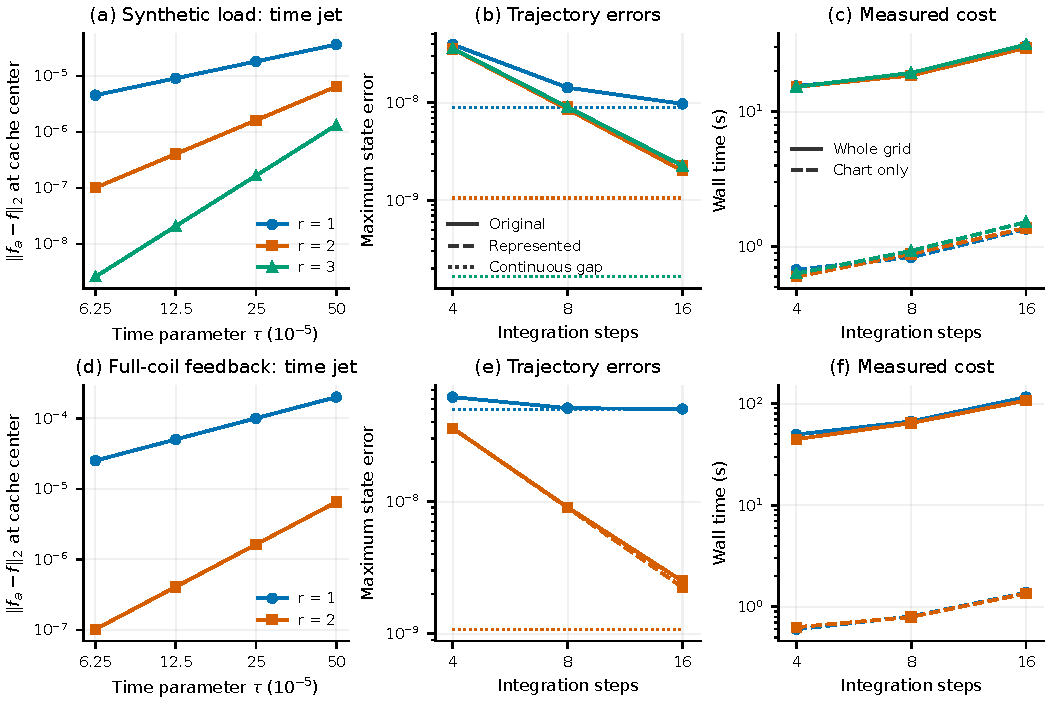
\includegraphics[width=\textwidth]{../figures/transport.pdf}
\caption{Accepted transport calculations. Rows correspond to the synthetic
load and full-coil collocated feedback. Left: native time-jet discrepancy at the
fixed cache center. Middle: sampled trajectory errors against the original
(solid) and represented (dashed) fields; dotted lines show continuous reference
gaps. Curves of represented errors nearly coincide. Right: complete grid wall
time and its auxiliary-chart component; coefficient and reference construction
are outside these per-grid timings. Color and marker identify transport order,
which does not change midpoint's second-order time discretization.}
\label{fig:transport}
\end{figure*}

\subsection{Direct integrators and failure domains}

Each direct-integrator branch has its own physical field and two independent
DOP853 references, using tolerances $(2\times10^{-11},2\times10^{-13},T/4)$
and $(5\times10^{-13},5\times10^{-15},T/8)$. Their reference refinement
differences are $1.24\times10^{-17}$, $8.01\times10^{-18}$, and
$1.38\times10^{-17}$ for fixed current, proportional drag, and collocated
feedback. All methods start at the same prescribed amplitude $0.01$, but errors
are compared only within a branch. The 15 method/grid combinations and 6
references took $690.713$\,s.

In the fixed-current conservative branch, midpoint and inherited nonseparable
Central4 attain finest errors $2.2449\times10^{-9}$ and
$1.4749\times10^{-13}$, with orders $1.9996$ and $3.9966$
(Figure~\ref{fig:integrators}). For synthetic proportional drag $-0.2P$, ordinary
and weighted midpoint are both second order, but only the weighted construction
targets $K(\tau)=e^{0.2\tau}K_0$. Its finest defect is
$1.11\times10^{-15}$, compared with $1.17\times10^{-9}$ for ordinary midpoint.
The actual collocated current law is evaluated at the unknown midpoint with
its full feedback Jacobian. Its canonical defect is $3.93\times10^{-4}$:
small integration residuals do not imply preservation of $K_0$. Central4 and
the proportional weighting are not applied to this general feedback branch.
Structure diagnostics use ideal implicit tangents at all midpoint steps, but
only the first Central4 step; floating-point maps are not asserted exactly
symplectic.

Locality is tested explicitly. Among 25 time-parameter chart probes, synthetic
order two at $\tau=0.2$, order three at $0.05$ and $0.2$, and full-coil order two
at $0.2$ leave the declared radius $0.002$ and are rejected. Two additional
outside-ball inputs are rejected as expected. These are auxiliary-chart probes,
not long robot trajectories. Polynomial nondegeneracy bounds lack directed
rounding and therefore are not interval certificates. The evidence establishes
short-window, smooth-field numerical connections; it does not establish chart
transitions, constrained sampled-feedback structure, long-time convergence, or
a new KAM certificate.

\begin{figure*}[t]
\centering
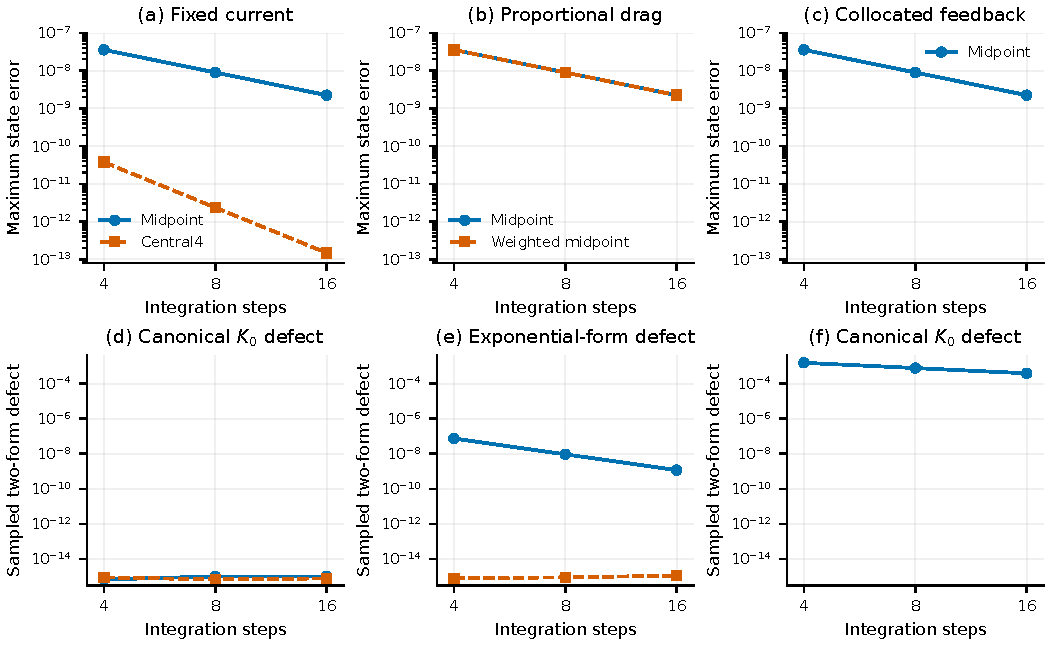
\includegraphics[width=\textwidth]{../figures/integrators.pdf}
\caption{Branch-specific direct integration. Top: errors against each branch's
own refined reference. Bottom: canonical two-form defects for fixed current and
collocated feedback, and the exponential two-form defect for proportional drag.
The two proportional-branch error curves nearly overlap. Defects sample ideal
implicit tangents, with only the first step sampled for Central4. The collocated
branch's nonzero canonical defect motivates a field-specific representation;
it does not invalidate its second-order trajectory convergence.}
\label{fig:integrators}
\end{figure*}
